\chapter{Wyniki eksperymentalne}
\thispagestyle{chapterBeginStyle}



\subsection{Środowisko testowe}



\section{Gęstość grafu}



\subsection{Problem przyrostowy}

\begin{figure}[!htbp]
	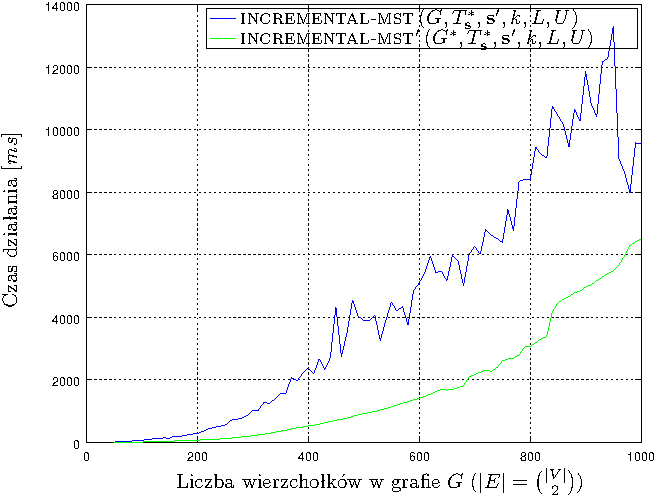
\includegraphics[width=\textwidth]{Chapter_VI/IMST1-example/IMST1_psfrag}
	\caption{
		cap
	}
	\label{fig:imst1}
\end{figure}

\begin{figure}[!htbp]
	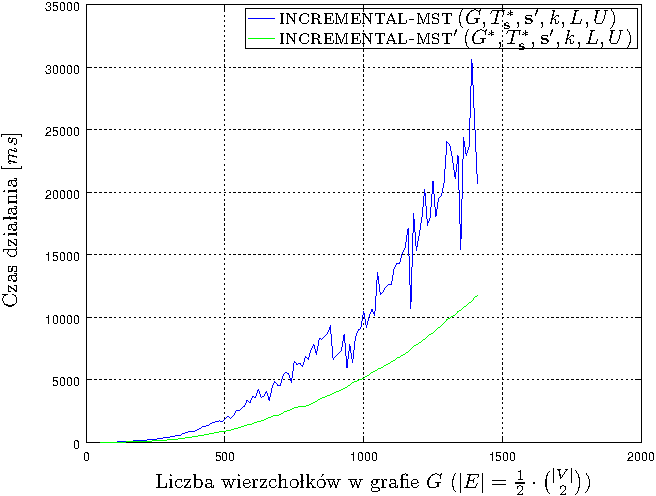
\includegraphics[width=\textwidth]{Chapter_VI/IMST2-example/IMST2_psfrag}
	\caption{
		cap
	}
	\label{fig:imst2}
\end{figure}

\begin{figure}[!htbp]
	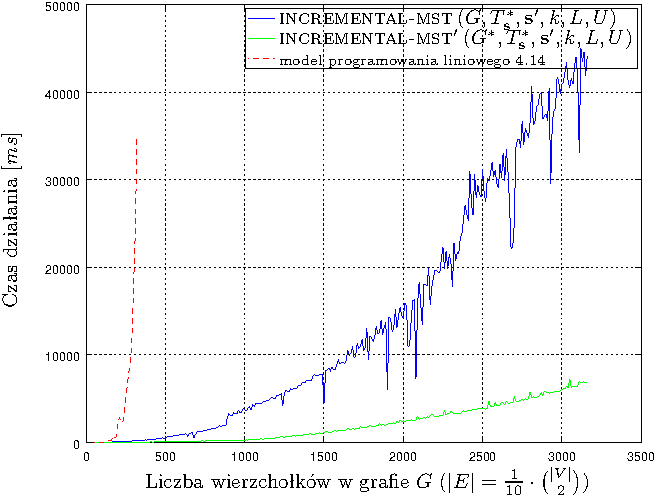
\includegraphics[width=\textwidth]{Chapter_VI/IMST3-example/IMST3_psfrag}
	\caption{
		cap
	}
	\label{fig:imst3}
\end{figure}

\begin{figure}[!htbp]
	\null\hfill
	\begin{subfigure}[b]{0.32\textwidth}
		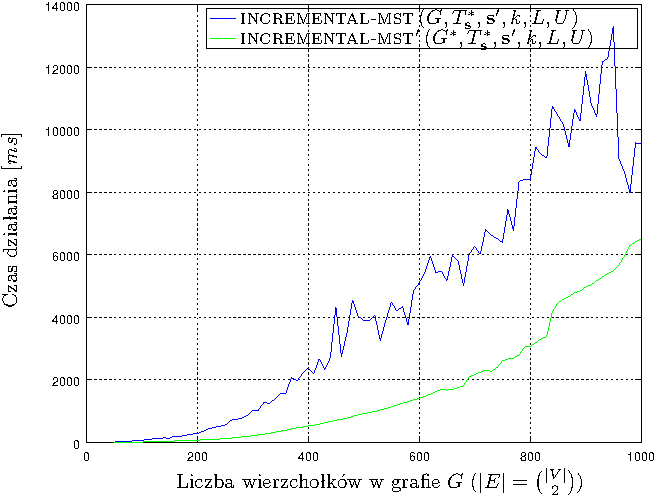
\includegraphics[width=\textwidth]{Chapter_VI/IMST1-example/IMST1_psfrag}
		\caption{}
		\label{fig:a:a}
	\end{subfigure}
	\hfill
	\begin{subfigure}[b]{0.32\textwidth}
		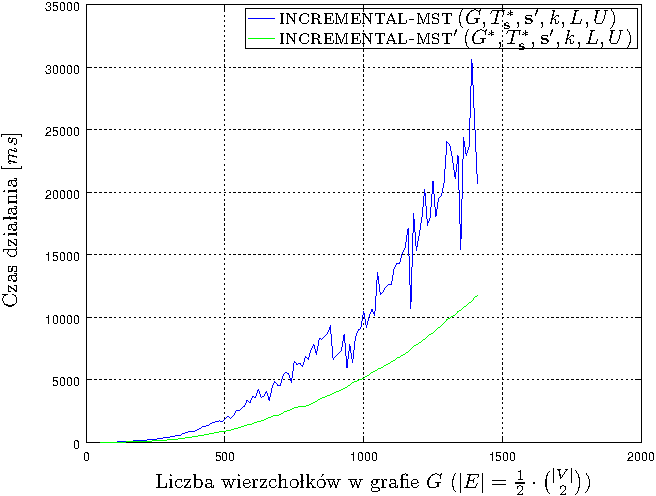
\includegraphics[width=\textwidth]{Chapter_VI/IMST2-example/IMST2_psfrag}
		\caption{}
		\label{fig:a:b}
	\end{subfigure}
	\hfill
	\begin{subfigure}[b]{0.32\textwidth}
		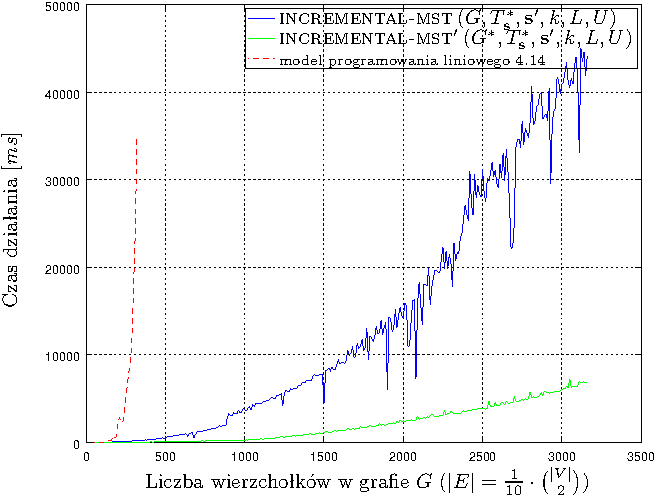
\includegraphics[width=\textwidth]{Chapter_VI/IMST3-example/IMST3_psfrag}
		\caption{}
		\label{fig:a:c}
	\end{subfigure}
	\hfill\null
	\caption{
		\textbf{(a)}~Nieskierowany graf $G = \left( V, E \right)$, gdzie $V = \left\{ v_{1}, v_{2}, \dots, v_{8} \right\}$ i $E = \left\{ e_{1}, e_{2}, \dots, e_{11} \right\}$.
		\textbf{(b)}~Skierowana wersja tego samego grafu.
	}
	\label{fig:a}
\end{figure}


\subsection{Wyniki i wykresy zależności}


\begin{figure}[!htbp]
	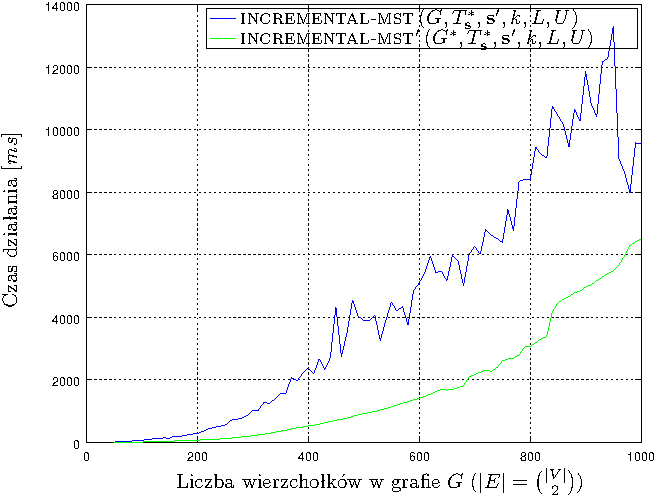
\includegraphics[width=\textwidth]{Chapter_VI/IMST1-example/IMST1_psfrag}
	\caption{
		cap
	}
	\label{fig:tabusearchGreedy}
\end{figure}
